\documentclass[../main.tex]{subfiles}
\graphicspath{{\subfix{../images/}}}
\begin{document}
\textbf{ Quelques Images du Thème}
    \begin{figure}[bh]
        \centering
        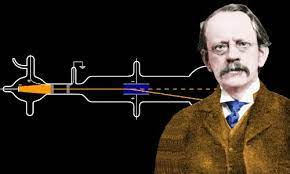
\includegraphics[width=7cm]{00.JJ-THOMSON} \caption{Lived 1856 – 1940} 
        \includegraphics[width=7cm]{00.JJ-THOMSON-LAB} 
        \caption{In His LAB}
        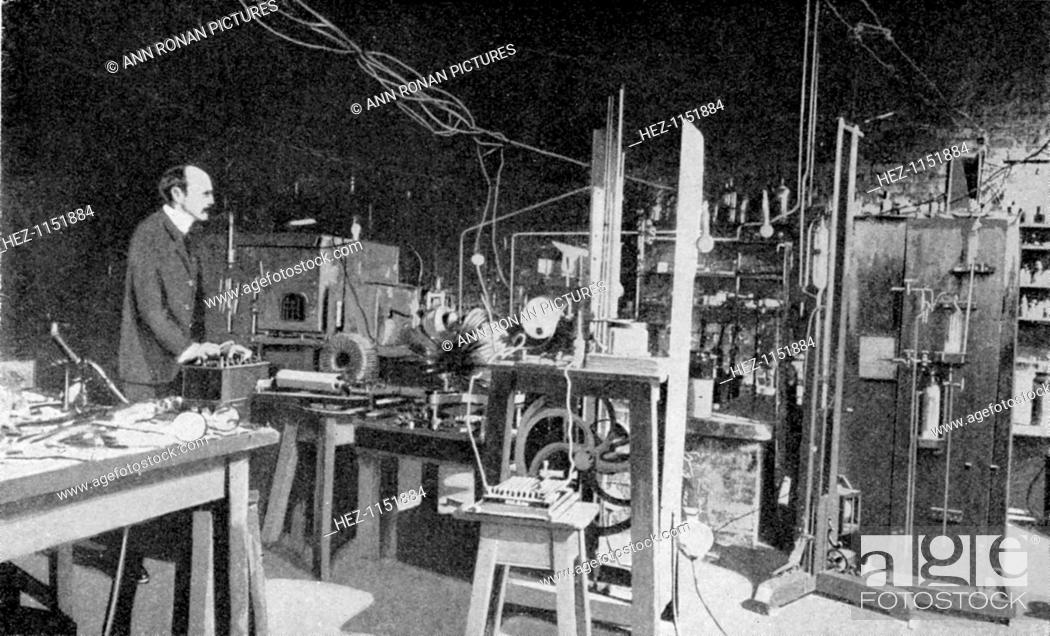
\includegraphics[width=7cm]{01.JJ-THOMSON-LAB} 
         \caption{In His LAB LARGE}
        \label{fig:img1}
        
    \end{figure}
    
    \begin{enumerate}
   \item First level item
   \item First level item
   \begin{enumerate}
     \item Second level item
     \item Second level item
     \begin{enumerate}
       \item Third level item
       \item Third level item
       \begin{enumerate}
         \item Fourth level item
         \item Fourth level item
       \end{enumerate}
     \end{enumerate}
   \end{enumerate}
 \end{enumerate}
    
    
\end{document}